\documentclass[../../main.tex]{subfiles}


\begin{document}

\subsection*{(a)}
The following screenshots show the process used for 4a). A minimum support count of 250 was specified in the task. At a dataset size of 4982 this equals a minimum support of $\frac{250}{4982}=0.05$\\
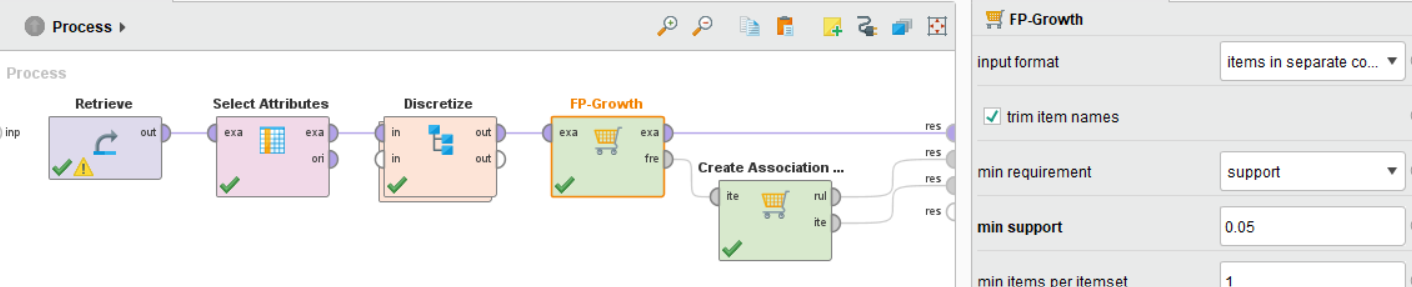
\includegraphics[width=\textwidth]{img/QUESTION_4a_PROCESS_overview.png}
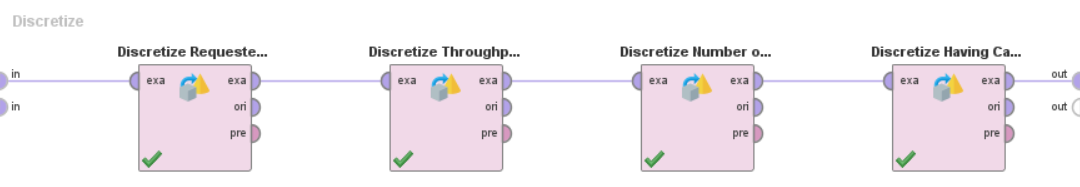
\includegraphics[width=\textwidth]{img/QUESTION_4a_PROCESS_discretize.png}
158 association rules were found at a minimum confidence of 0.8, the top 10 in confidence can be seen below:\\
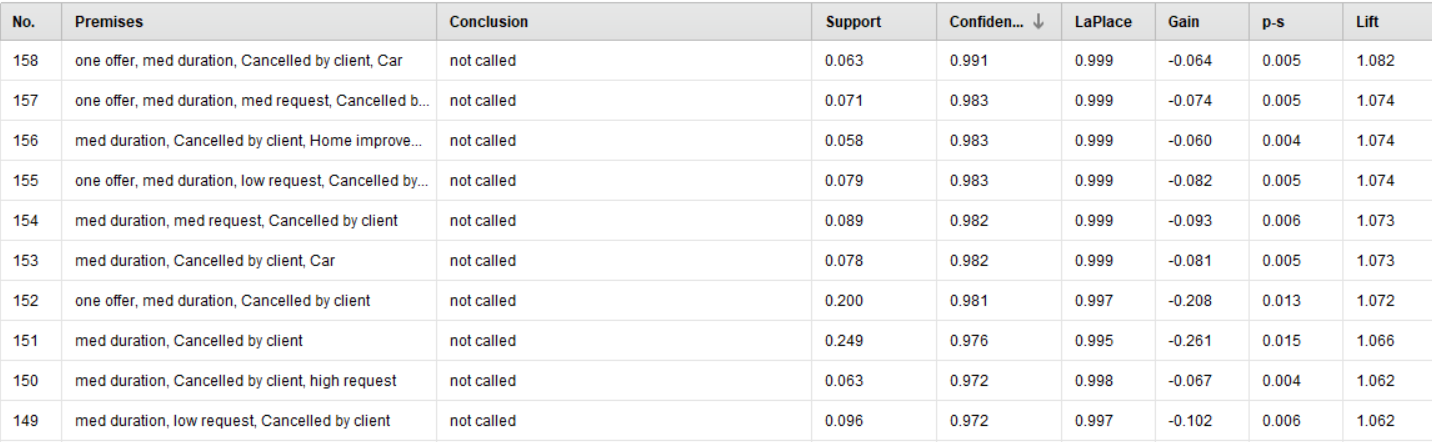
\includegraphics[width=\textwidth]{img/QUESTION_4a_association_rules.png}

\subsection*{(b)}
The conclusion with the highest confidence (0.991) states that if there is a car loan with one offer and a medium throughput time that gets cancelled by the client, the client likely doesn't call to complete the application. However this association rule is not very interesting to the bank manager due to its low support of just $\sim6\%$\\
The conclusion with the lowest confidence in our analysis (0.8) states that if an application had a medium duration and was cancelled by the client there was likely just one offer. This rule has a fairly good support of 20\% and lift larger than one, therefore it might theoretically be interesting to the bank manager. However it does not state any useful new facts besides that when an application is cancelled by the client after a medium time there usually aren't many offers to be made.



\end{document}